\section{Test}
\label{sec:Test}

Die Anwendung ist nach Abschluss der Umsetzungsphase fertiggestellt und
einsatzbereit. Vor Projektabschluss und -übergabe soll die Software auf ihre
Qualität geprüft werden. Es soll darüber hinaus verifiziert werden, dass alle
Anforderungen des Lastenheftes umgesetzt wurden. Sowohl die Qualität der
Anwendung, als auch die Umsetzung aller Anforderungen werden im Folgenden in
einem zweistufigen Praxistest der Software überprüft.

Im ersten Schritt wird die Software einem Alphatest unterzogen. Ein Alphatest
liegt hierbei vor, wenn der Test von Personen durchgeführt wird, welche an
der Entwicklung des zu testenden Produktes beteiligt waren. In diesem Fall
wird der Alphatest also vom Projektteam durchgeführt. In dem Alphatest werden
vor allem die in \verweis{Lastenheft} genannten Produktfunktionen des
Lastenhefts überprüft. In dem Test sollen erste grobe Fehler in Bedienung,
Anzeige und Verhalten identifiziert werden und es soll zusätzlich sichergestellt
werden, dass alle Anforderungen des Auftraggebers umgesetzt wurden. Die Tests
der Produktfunktionen werden in den vier führenden Browsern\footnote{Quelle:
\url{http://www.chip.de}} Chrome, Firefox, Internet Explore und Safari
durchgeführt, um browserübergreifende Funktionalität sicherzustellen.
Dabei werden die Testbereiche Bedienung, Anzeige und Verhalten untersucht. Das
Ergebnis des durchgeführten Alphatests ist in \abbildung{Alphatest} dargestellt.

\begin{figure}[htb]
\centering
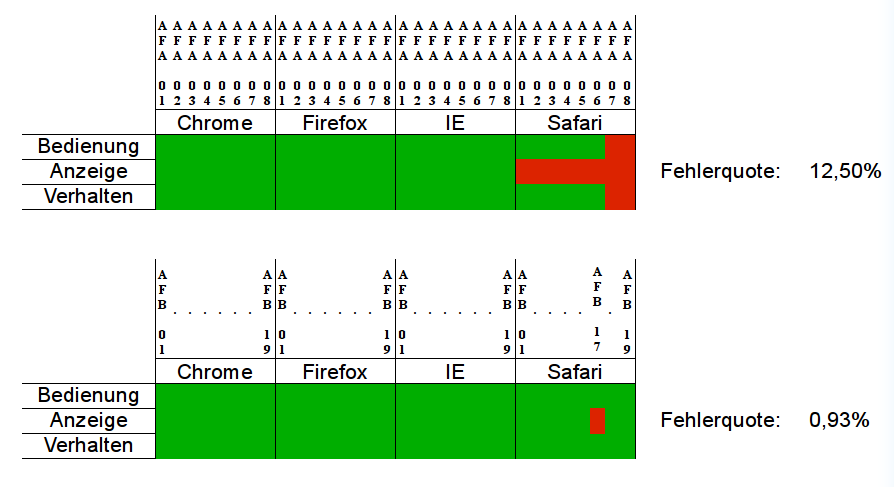
\includegraphics[width=1.0\textwidth]{Alphatest.png}
\caption[Graphische Darstellung des Alphatests]{Graphische Darstellung des Alphatests\protect\footnotemark}
\label{fig:Alphatest}
\end{figure}
\footnotetext{Quelle: Eigene Darstellung}

Die Auswertung des Alphatests zeigt, dass alle Anforderungen in der
Anwendung umgesetzt wurden. Darüber hinaus traten in keinem der geprüften
Anwendungsfälle Fehler auf. Es zeigten sich jedoch beim Vergleich der
verschiedenen getesteten Browser deutliche Unterschiede in der
Darstellungsgeschwindkeit. Das Umsehen in den einzelnen Panoramafotos stellt
sich so im Chrome-Browser flüssiger als im Internet Explorer oder im
Firefox dar. Aus diesem Grund wird der Chrome-Browser für die Benutzung der
Anwendung empfohlen.

Neben browserspezifischen Darstellungsunterschieden konnten in dem Alphatest
auch kleinere Schwachstellen der Anwendung gefunden werden, die nicht in den
Anwendungsfällen berücksichtigt wurden. Als Beispiel hierfür kann die falsche
Verlinkung einer Datei oder das Fehlen einer Sicherheitsabfrage beim Löschen
eines Datensatzes angeführt werden. Diese Mängel wurden im Anschluss an den
Alphatest direkt beseitigt. An dem Ergebnis des Alphatests wird aus der Sicht
des Projektteams der funktionale Erfolg der Anwendung deutlich.

Im zweiten Schritt der Testphase wird die Software einem Betatest unterzogen.
Dieser Betatest wird von Personen durchgeführt, die nicht an der Entwicklung der
Anwendung beteiligt waren. Der Test wurde durchgeführt um weitere Fehler in der
Software zu identifizieren. Weiterhin sollen durch den Betatest auch die
Projektziele verifiziert werden. Die Verifikation der Projektziele durch den
Betatest ist in der vorliegenden Projektbetrachtung jedoch nicht relevant und
wird daher nicht weiter vertieft. Diese kann jedoch in der Ausarbeitung
"`Unternehmensführung"'\footnote{\citet{unternehmensfuehrung2014}} nachgelesen
werden. 

Die Folgende Auflistung zeigt Fehler und Verbesserungsvorschläge, welche von
Betatestern geäußert wurden:

\begin{itemize}
  \item Ausführlichere Erklärungen zur Anwendung
  \item Optimierte Darstellung für mobile Endgeräte
  \item Einrichtung eines Hilfe-Buttons
  \item Erstellung einer Übersichtskarte aus Vogelperspektive
  \item Einführung von Tastenkürzeln zum Navigieren
\end{itemize}

Aufbauend auf dem hier nur verkürzt dargestellten Feedback der Betatester wird
ein weiterer Entwicklungszyklus begonnen, in dem diese Kritik ausgebessert wird.
Nicht jede Kritik kann dabei berücksichtigt werden. So kann beispielsweise die
verbesserte Darstellung für mobile Endgeräte im Rahmen des Projektstudiums nicht
mehr umgestetzt werden, da hierfür ein zu großer Entwicklungsaufwand nötig wäre.

Neben der Fehleranalyse wird, analog zu dem Alphatest, auch im Betatest ein
besonderer Fokus auf den Erfolg des Projektes aus Sicht der Betatester gelegt.
Hierzu ist in \abbildung{Betatest} eine subjektive Bewertung des Projektes aus
Sicht der Betatester dargestellt.

\begin{figure}[htb]
\centering
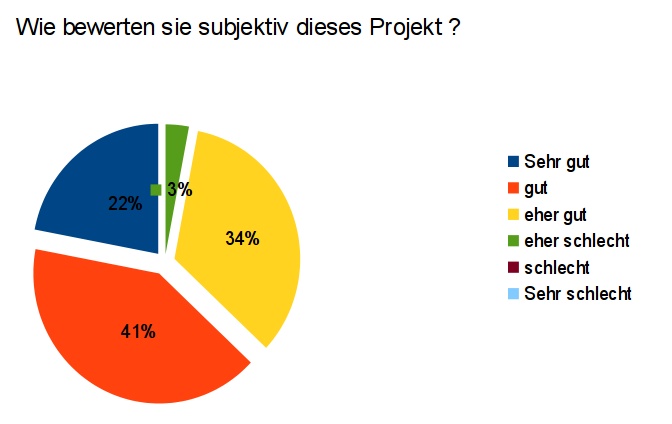
\includegraphics[width=1.0\textwidth]{Betatest.png}
\caption[Erfolg des Projektes aus Sicht der Betatester]{Erfolg des Projektes aus Sicht der Betatester\protect\footnotemark}
\label{fig:Betatest}
\end{figure}
\footnotetext{Quelle: Eigene Darstellung}

Sowohl aus Sicht des Entwicklerteams als auch aus Sicht der Betatester erfüllt
das Projekt am Ende der Testphase die zu Beginn des Projektes definierten
Anforderungen. Darüber hinaus wurde von den Betatestern viel positive
Rückmeldung zu dem Projekt geäußert.
